\documentclass[a4paper,12pt]{article}

\usepackage[utf8]{inputenc}
\usepackage[T1]{fontenc}
\usepackage[polish]{babel}
\usepackage{amsmath}
\usepackage{graphicx}
\graphicspath{{plots/}}
\usepackage{tikz}
\usetikzlibrary{trees}
\usepackage{float}
\usepackage{geometry}
\usepackage{hyperref}
\usepackage{array}

\geometry{margin=2.5cm}

\title{Algorytmy i Struktury Danych \\ Lista 3}
\author{}
\date{}

\begin{document}
\maketitle

\section{Wstęp}

W ramach zadania zaimplementowano oraz przetestowano kilka algorytmów. 

Dla algorytmów wykonano testy mierzące liczbę porównań (\texttt{cmp})
oraz przypisań (\texttt{assign}) w zależności od rozmiaru danych wejściowych.
Wyniki zaprezentowano na wykresach.

\section{CUT\_ROD}

Problem CUT\_ROD był testowany w trzech wersjach: naiwnej, ze spamiętywaniem
oraz iteracyjnej. Już na etapie generowania danych było widać, że wersja
naiwna bardzo szybko przestaje być użyteczna. Już dla rozmiaru 30 nie dałem rady doczekać na wynik.
Na wykresach maksymalnie przedstawiono przypadek \texttt{n=20}.


\subsection{Wyniki}

\begin{figure}[H]
    \centering
    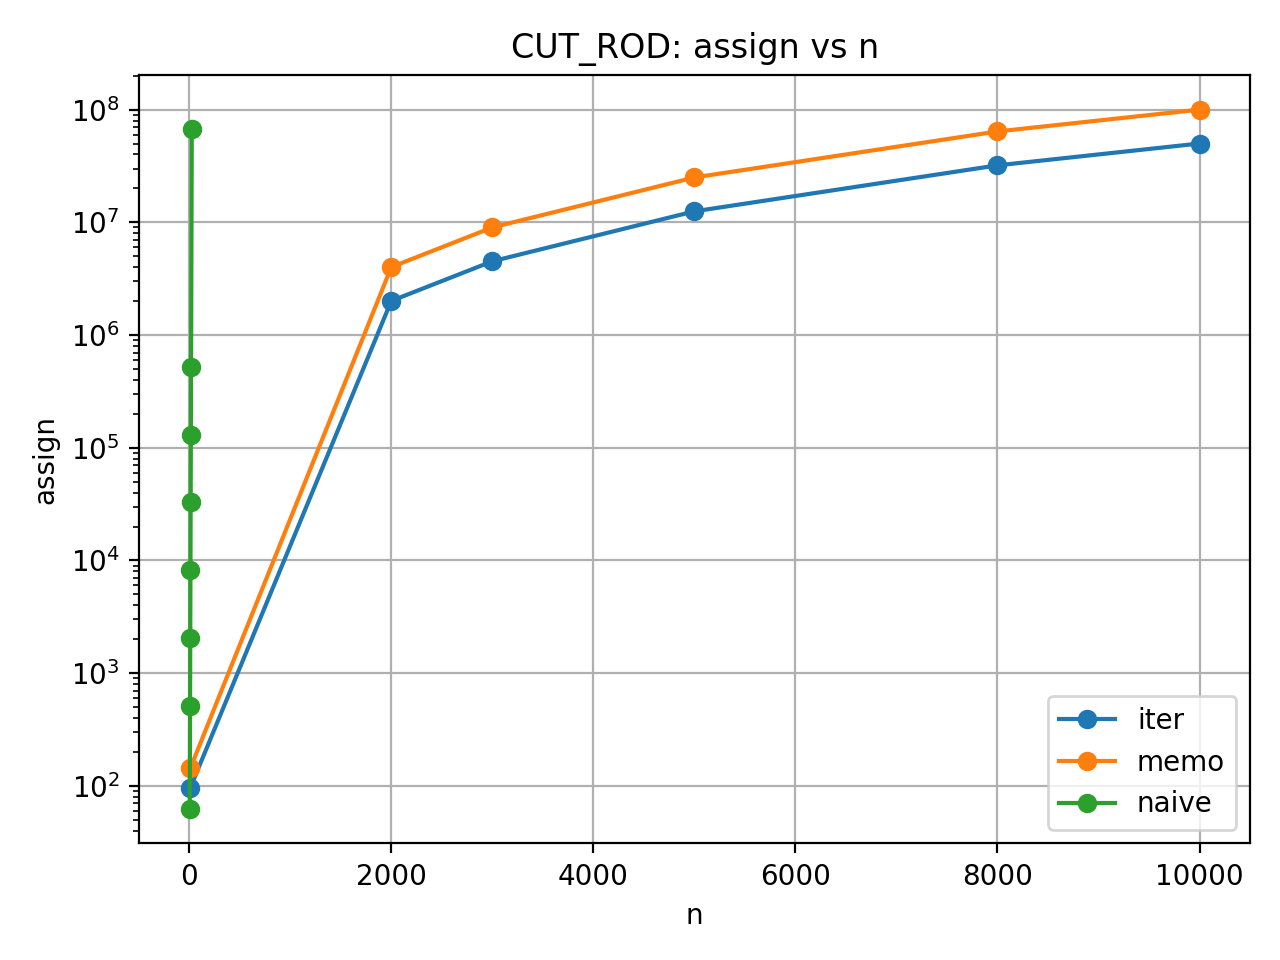
\includegraphics[width=0.85\textwidth]{CUT_ROD_assign.png}
    \caption{CUT\_ROD: liczba przypisań}
\end{figure}

\begin{figure}[H]
    \centering
    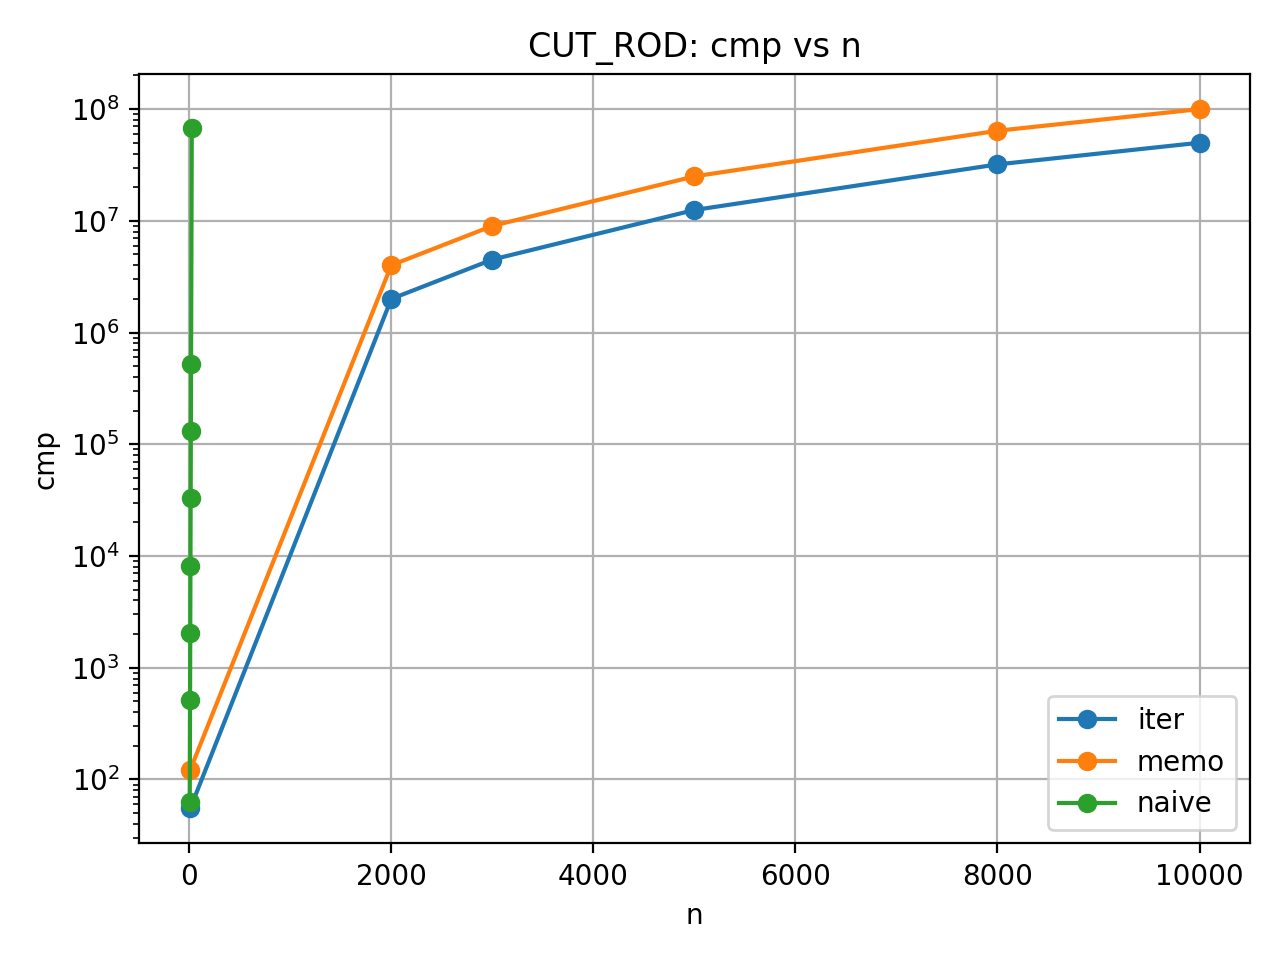
\includegraphics[width=0.85\textwidth]{CUT_ROD_cmp.png}
    \caption{CUT\_ROD: liczba porównań}
\end{figure}

Zastosowano skalę logarytmiczną, ponieważ wersja naiwna rośnie wykładniczo
i bardzo szybko „ucieka” na wykresach w porównaniu do pozostałych wersji.

\subsection{Komentarz}

Wersje ze spamiętywaniem oraz iteracyjna zachowują się stabilnie i rosną
w przewidywalny sposób. Wersja naiwna działa poprawnie tylko dla bardzo
małych danych i ma głównie znaczenie teoretyczne. Ciekawe jest, że wersja iteracyjna zachowuje się trochę
lepiej niż wersja ze spamiętywaniem, co może wynikać z mniejszej
ilości wywołań funkcji i związanych z tym narzutów.

\section{LCS}

Algorytm LCS został zaimplementowany w wersji rekurencyjnej ze spamiętywaniem
oraz iteracyjnej. Obie wersje mają złożoność kwadratową, dlatego różnice
pomiędzy nimi są mniejsze niż w przypadku CUT\_ROD.

\subsection{Wyniki}

\begin{figure}[H]
    \centering
    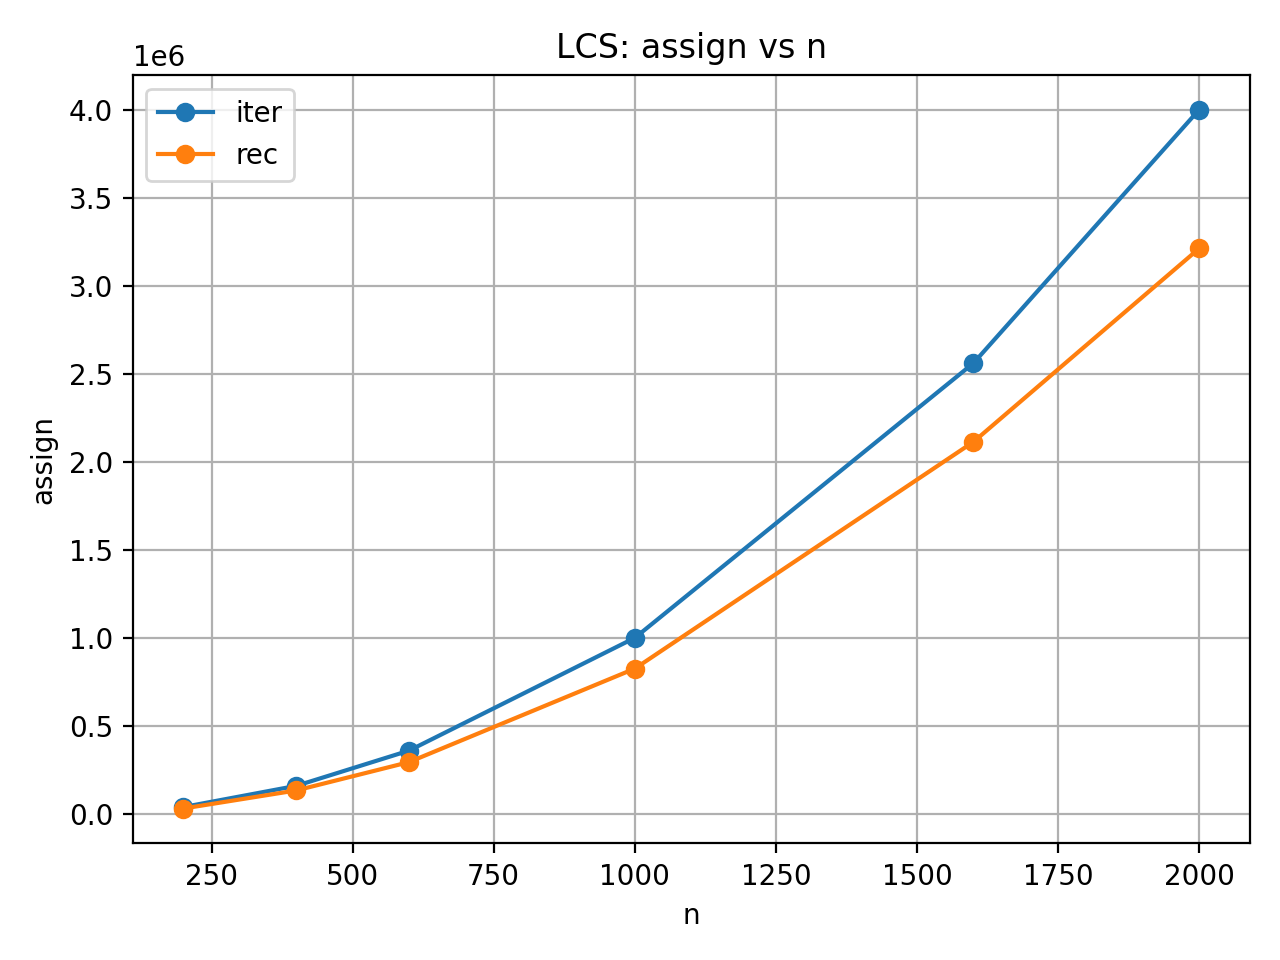
\includegraphics[width=0.85\textwidth]{LCS_assign.png}
    \caption{LCS: liczba przypisań}
\end{figure}

\begin{figure}[H]
    \centering
    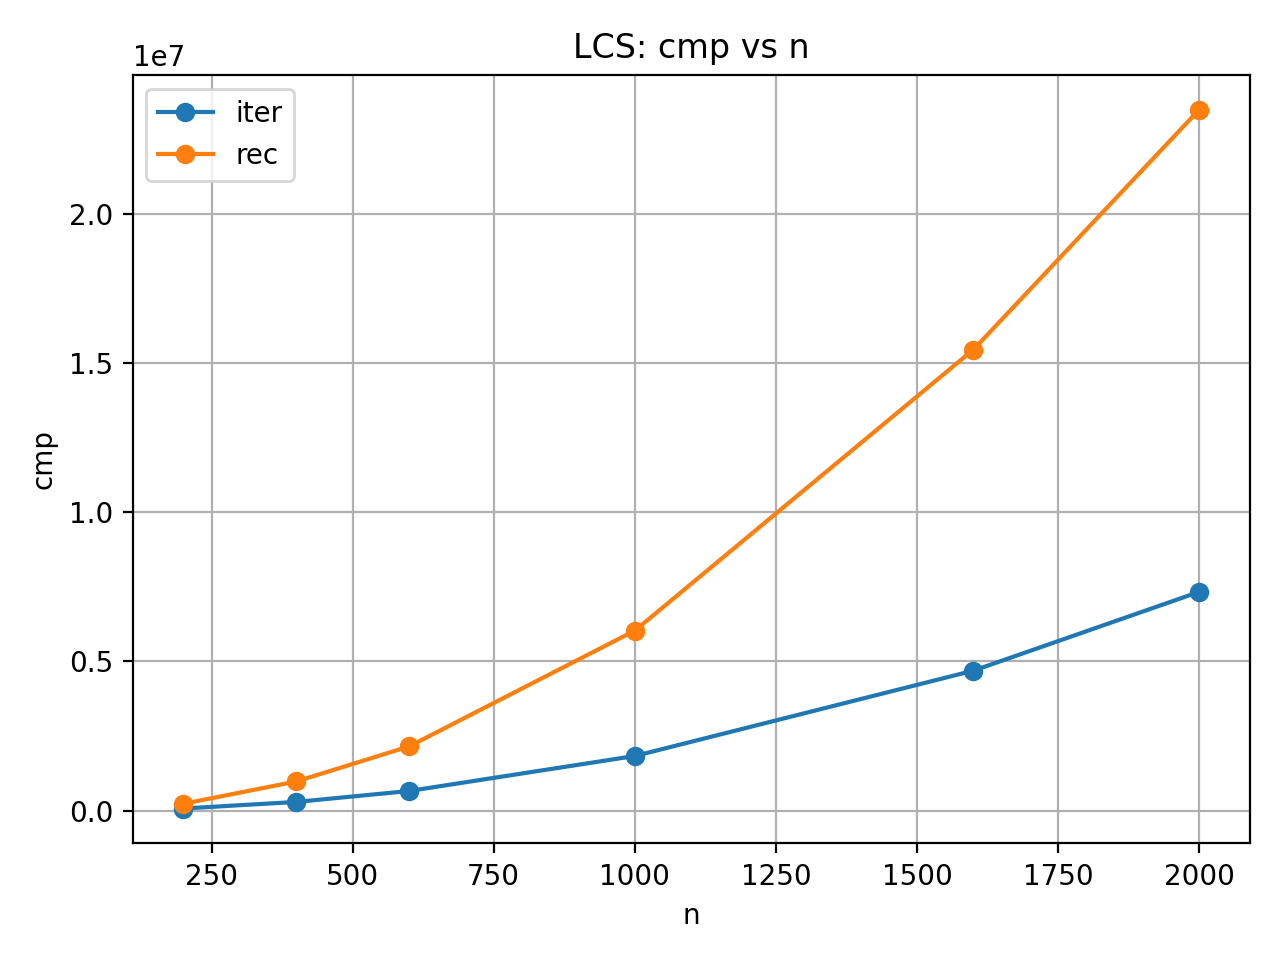
\includegraphics[width=0.85\textwidth]{LCS_cmp.png}
    \caption{LCS: liczba porównań}
\end{figure}

\subsection{Komentarz}

Wersja iteracyjna wykonuje mniej operacji niż wersja rekurencyjna, jeśli liczymy sumę przypisywań
i porównań, co jest
widoczne szczególnie dla większych danych. Ciekawe jest natomiast to, że w zależności od tego,
co jest w danym momencie ważniejsze, można wybrać odpowiednią wersję.
Różnice nie są jednak bardzo
duże, ponieważ oba algorytmy rosną zgodnie z oczekiwaną złożonością
$O(n^2)$.

\section{ACTIVITY\_SELECTOR}

Dla problemu wyboru aktywności zaimplementowano trzy wersje: rekurencyjną,
iteracyjną oraz dynamiczną o złożoności kwadratowej.

\subsection{Wyniki}

\begin{figure}[H]
    \centering
    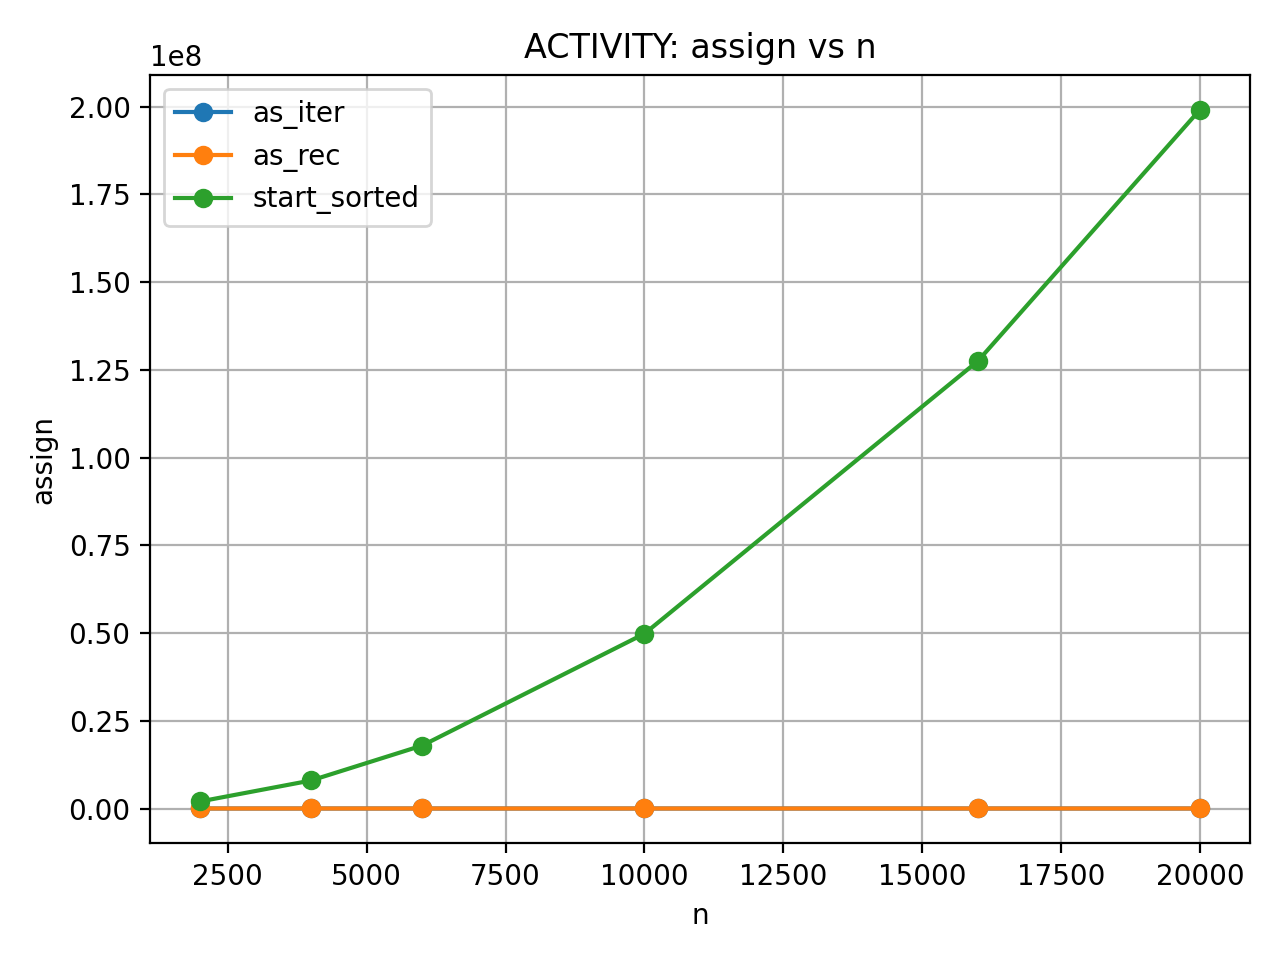
\includegraphics[width=0.85\textwidth]{ACTIVITY_assign.png}
    \caption{ACTIVITY: liczba przypisań}
\end{figure}

\begin{figure}[H]
    \centering
    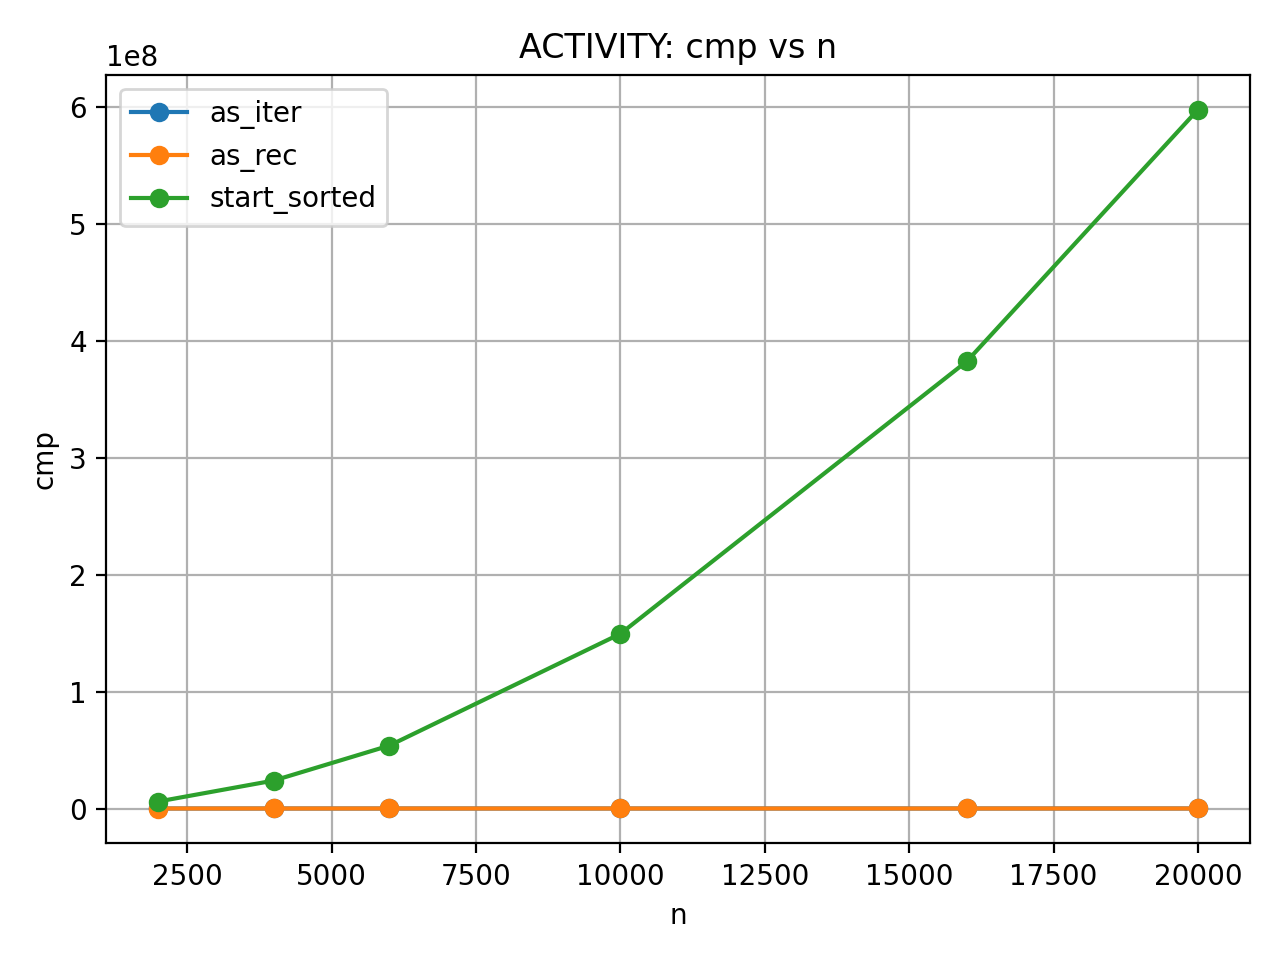
\includegraphics[width=0.85\textwidth]{ACTIVITY_cmp.png}
    \caption{ACTIVITY: liczba porównań}
\end{figure}

Algorytm dynamiczny bardzo szybko zaczyna wychodzić poza wykres, bo ma złożoność kwadratową, dlatego
dodatkowo pokazano porównanie tylko dwóch szybkich wersji.

\begin{figure}[H]
    \centering
    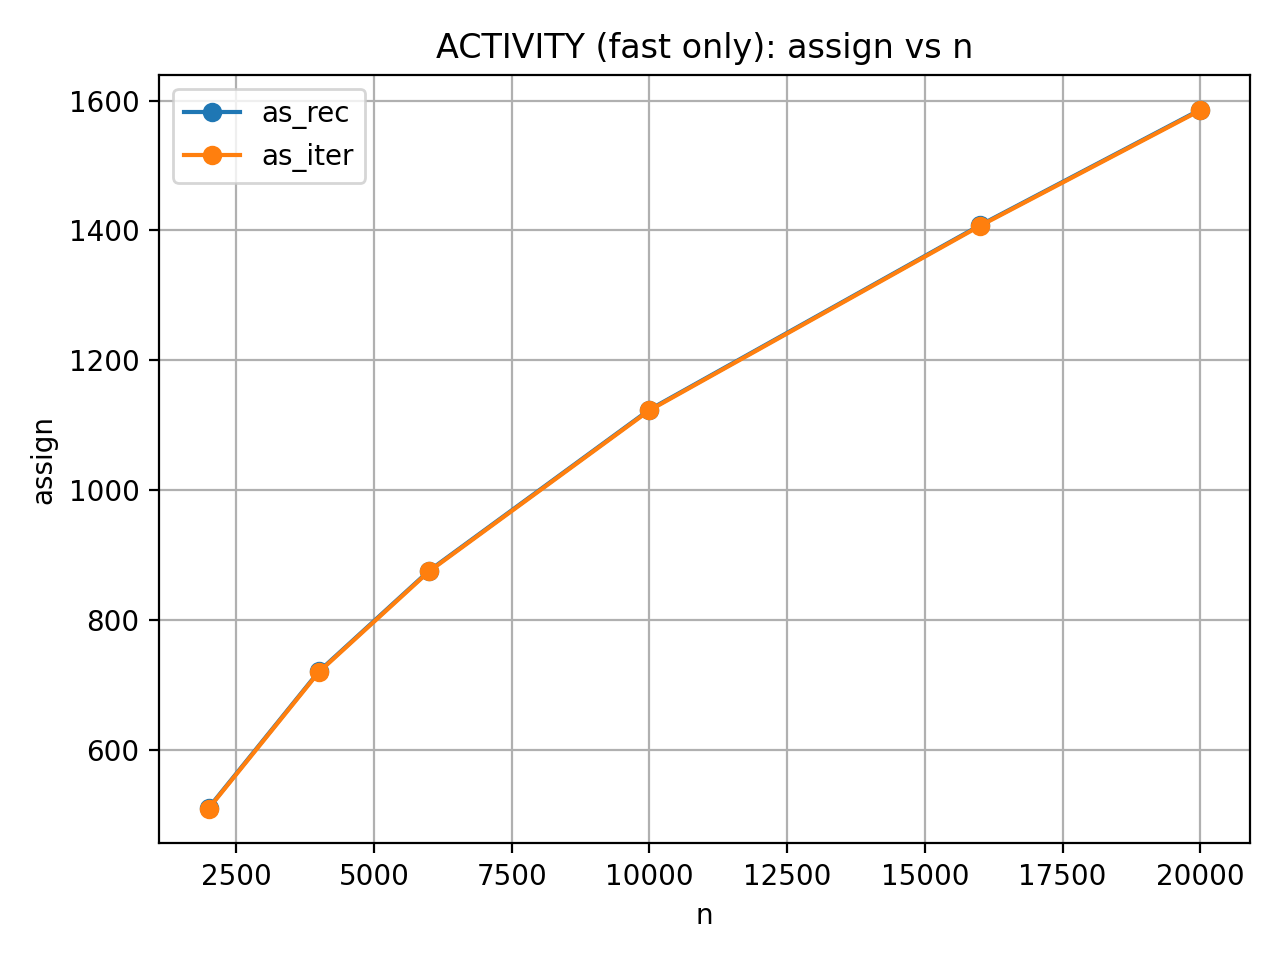
\includegraphics[width=0.85\textwidth]{ACTIVITY_fast_assign.png}
    \caption{ACTIVITY (szybkie wersje): liczba przypisań}
\end{figure}

\begin{figure}[H]
    \centering
    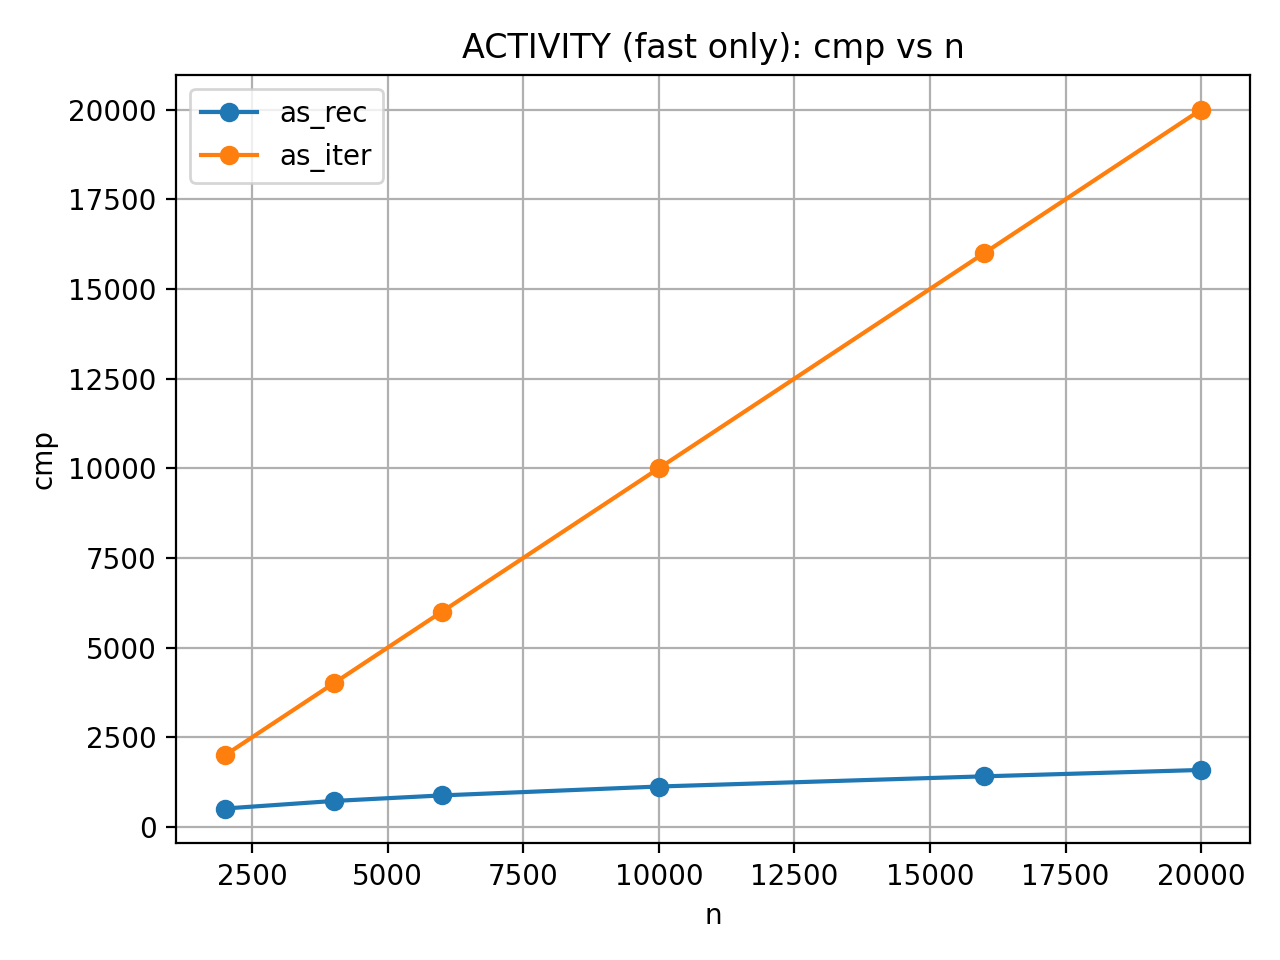
\includegraphics[width=0.85\textwidth]{ACTIVITY_fast_cmp.png}
    \caption{ACTIVITY (szybkie wersje): liczba porównań}
\end{figure}

\subsection{Komentarz}

Rozwiązanie dynamiczne bardzo szybko staje się niepraktyczne. Ciekawe jest, że wersja rekurencyjna i
iteracyjna zachowują się nawet nie podobnie, a identycznie w przypadku liczby przypisań,
ale różnią się w liczbie porównań, gdzie wersja iteracyjna jest zauważalnie
wolniejsza. 

Ale chcę podkreślić, że wersja bazująca na zajęciach posortowanych według
czasu rozpoczęcia jest mniej szybka dlatego, że taki algorytm jest sam w sobie
bardziej złożony.

\section{Algorytm Huffmana}

Algorytm Huffmana w wersji ternarnej wydaje się być najbardziej interesującym
elementem całego zadania. Jak najbardziej ciekawe było znalezienie idei z dodawaniem 
kilku elementów pustych, aby drzewo mogło być poprawnie zbudowane.

\begin{figure}[H]
\centering
\begin{tikzpicture}[
  level distance=16mm,
  sibling distance=40mm,
  edge from parent/.style={draw, -latex},
  every node/.style={draw, rounded corners, align=center, font=\small, inner sep=2.5pt}
]
\node {root}
  child { node {a\\\texttt{0}} edge from parent node[midway, left, draw=none]{\texttt{0}} }
  child { node {g\\\texttt{1}} edge from parent node[midway, left, draw=none]{\texttt{1}} }
  child { node {$\bullet$}
    child { node {b\\\texttt{20}} edge from parent node[midway, left, draw=none]{\texttt{0}} }
    child { node {e\\\texttt{21}} edge from parent node[midway, left, draw=none]{\texttt{1}} }
    child { node {$\bullet$}
      child { node {d\\\texttt{220}} edge from parent node[midway, left, draw=none]{\texttt{0}} }
      child { node {f\\\texttt{221}} edge from parent node[midway, left, draw=none]{\texttt{1}} }
      child { node {c\\\texttt{222}} edge from parent node[midway, left, draw=none]{\texttt{2}} }
      edge from parent node[midway, left, draw=none]{\texttt{2}}
    }
    edge from parent node[midway, left, draw=none]{\texttt{2}}
  };
\end{tikzpicture}
\caption{Drzewo Huffmana (ternarne) dla tekstu \texttt{"aaaaaaabbbccdeeeeffggggggggg"}}
\end{figure}

Liczba kodowanych symboli powinna być nieparzysta, bo w innym przypadku algorytm może zostawić
pustą krawędź, co nie jest optymalne.

Algorytm ten był szczególnie ciekawy podczas implementacji i testów,
ponieważ nawet dla krótkiego tekstu struktura drzewa i przypisane kody
nie są oczywiste na pierwszy rzut oka.

\section{Porównanie algorytmów}

\begin{center}
\begin{tabular}{|>{\raggedright}p{4cm}|c|c|}
\hline
\textbf{Algorytm} & \textbf{Szybkość} & \textbf{Komentarz} \\
\hline
CUT\_ROD (naiwny) & bardzo wolny & szybko przestaje mieć sens \\
\hline
CUT\_ROD (iter lub memo) & szybki  & stabilne zachowanie \\
\hline
LCS & szybki & rośnie kwadratowo \\
\hline
ACTIVITY (iter lub rec) & bardzo szybki & najlepszy wybór w praktyce \\
\hline
ACTIVITY (start sorted) & wolny  &jeśli sortowanie danych jest kosztowne\\
\hline
Huffman & szybki  & najbardziej „niezwykły” algorytm \\
\hline
\end{tabular}
\end{center}

\section{Podsumowanie}

Na podstawie wykresów i testów można zauważyć, że algorytmy naiwne lub
kwadratowe bardzo szybko przestają być użyteczne dla większych danych.
Zastosowanie spamiętywania lub iteracji daje
znaczną poprawę wydajności.

Algorytm Huffmana wyróżnia się tym, że oprócz analizy złożoności pozwala
na obserwację konkretnego efektu działania algorytmu, co czyni go
najbardziej „wizualnym” elementem całego zadania.

\end{document}
